%%%%%%%%%%%%%%%%%%%%%%%%%%%%%%%%%%%% 
% This is the template for submission to ISCA 2018
% The cls file is a modified from  'sig-alternate.cls'
%%%%%%%%%%%%%%%%%%%%%%%%%%%%%%%%%%%% 

\documentclass{sig-alternate} 
\usepackage{mathptmx} % This is Times font

\newcommand{\ignore}[1]{}
\usepackage{fancyhdr}
\usepackage[normalem]{ulem}
\usepackage[hyphens]{url}
\usepackage{microtype}
\usepackage{graphicx}

% Ensure letter paper
\pdfpagewidth=8.5in
\pdfpageheight=11in


\newcommand{\iscasubmissionnumber}{4}

\fancypagestyle{firstpage}{
  \fancyhf{}
  \renewcommand{\headrulewidth}{0pt}
  \fancyhead[C]{\normalsize{In-Class CBP Submission
      \textbf{\#\iscasubmissionnumber} \\ Confidential Draft: DO NOT DISTRIBUTE}} 
  \fancyfoot[C]{\thepage}
}  

\pagenumbering{arabic}

\title{Branch Predictor - Group 4} 
\author{Subhdeep Saha (150732) | Yash Srivastav (150839)}

% Always include hyperref last
\usepackage[bookmarks=true,breaklinks=true,letterpaper=true,colorlinks,linkcolor=black,citecolor=blue,urlcolor=black]{hyperref}


\begin{document}
\maketitle
\thispagestyle{firstpage}
\pagestyle{plain}

\begin{abstract}

  This paper describes a branch predictor developed for the in-class Championship
  Branch Prediction of CS422 (2017-18-II). The base target of this branch predictor
  was to perform better than the gshare branch predictor \cite{combine-bp}.

  We introduce a branch predictor based on the GEHL Predictor introduced in \cite{ogehl}
  augmented with a side predictor (the loop predictor).

  This augmentation with a loop predictor is fairly common and has been used in
  \cite{ltage} and \cite{tagescl} for augmenting the TAGE Predictor.
\end{abstract}

\subsection*{Paper outline}

The remainder of the paper is organized as follows.
Section \ref{sec-framework} details the evaluation framework used.
Section \ref{sec-predictor} introduces the predictor and its design.
Section \ref{sec-analysis} explores the design space and decisions
taken while choosing parameters.
Section \ref{sec-summary} reviews related work and summarizes
this study.

\section{Evaluation Framework}
\label{sec-framework}

We have used the Evaluation Framework used for the 1st CBP. The following
traces have been used for measuring the accuracy of our branch predictor:

\begin{itemize}
\item INT-1
\item INT-2
\item INT-3
\item MM-1
\item MM-2
\item SERV-1
\item SERV-2
\item SERV-3
\item SERV-4
\item SERV-5
\end{itemize}

\section{Predictor}
\label{sec-predictor}

The predictor consists of $N$ tables indexed by different history lengths.
The results of each individual table are combined using an adder-tree and
the final result is considered to be the prediction of the gehl predictor.

Now, based on whether there was a hit or not in the loop predictor, a bimodal
predictor is used to select between the loop predictor and the gehl predictor.

\subsection{Tables}

There are $N$ tables, having $E(i)$, $1 \leq i \leq N$, entries each. Each entry
consists of a $C(i)$, $1 \leq i \leq N$, bit signed saturating counter used to provide a
bimodal prediction.

We calculate a sum like the following:
\begin{equation}
  sum = \sum_{i=1}^{N} Pred(i) / C(i)
\end{equation}

The sign of the sum determines the direction to be taken.

In order to prevent floating values at a hardware level, the sum can be
calculated as:

\begin{equation}
  sum = \sum_{i=1}^{N} \frac{\left( Pred(i) \times {\displaystyle \prod_{j=1}^{N}C(j)} \right)}{C(i)}
\end{equation}

\subsection{Preventing Path Aliasing}

For computing the indexes for global history predictors,
most studies consider either hashing the conditional branch
history with the branch address or hashing the path history
with the branch address. In both of these cases, we consider
some paths as equal even before computing the effective
index in the predictor tables. This phenomenon is called path aliasing.
The impact of path aliasing on predictor
accuracy is important when a short global
history is used.

As discussed in \cite{ogehl}, in order to limit this phenomenon,
we include nonconditional branches in the branch history (inserting
a taken bit) and we also record a path history consisting
of 1 address bit per branch.

Since effect of path aliasing decreases with increasing history length,
we only need to maintain a short path history.

\subsection{Indexing}

Each table $T_i$ is indexed with different global history lengths $L(i)$ and
other parameters like path history and Program Counter. Our indexing function
does the following for a table containing $2^m$ entries ($m$-bit index):
\begin{itemize}
  \item Start with $Min(L(i), 16)$ bits of Path History
  \item Append $L(i)$ bits of Global History
  \item Append PC bits
  \item Now, break this up into groups of $m$ bits and xor them all together
  \item If the number of bits are not a multiple of $m$, append $0$s (xor identity).
  \item The obtained $m$ bit value is the index.
\end{itemize}

The above kind of ``rollover" indexing is also used in \cite{cbp1.5}.

\subsection{Loop Predictor}

A loop predictor tries to identify regular loops with fixed number of iterations.
The following parameters are associated with an entry in the loop predictor:
\begin{itemize}
  \item Past Iterations - The total number of iterations taken in the past
  \item Confidence - The confidence in the loop predictor (a counter)
  \item Current Iterations - The number of iterations currently completed
  \item Tag - A unique tag for identifying entries in the predictor
  \item Age - Age of the loop predictor. Used in replacement policies.
  \item Dir - The Direction supposed to be taken in general in the loop.
\end{itemize}

Every time a branch is encountered, it is considered for placement in the loop
predictor table with low probability. Since loop branches occur many times, they
have a high probability of being allocated an entry.

Once an entry is allocated, the branch's behaviour is matched up with that of a
loop. Every time, it exhibits loop behaviour, the confidence associated with it
is incremented. Once the confidence counter is saturated, we consider the
results of the loop predictor while predicting branch direction.

The Age counter (saturating unsigned counter) is incremented/decremented
depending upon conditions. Every time a loop predictor is a possible replacement
entry, the age is decremented. Every time the loop predictor predicts correctly,
the age is incremented. If there is a misprediction/the branch is identified as
not being a loop, the age is reset to 0. While replacing, only entries with age
0 can be replaced.

A separate signed counter (WITHLOOP) is maintained for determining whether loop
predictions are being useful or not. Whenever a loop prediction gives correct
prediction as compared to our gehl predictor, the counter is incremented.
Whenever it gives the wrong prediction, the counter is decremented. If the
counter is positive, then only we consider loop predictions.

\subsection{Prediction}

The prediction is quite simple. First we obtain the gehl prediction. Then,
if WITHLOOP > 0 and there is a hit in the loop predictor with enough confidence,
then the loop prediction is used.

\subsection{Predictor Update}

Once a branch is completed, and we know the results of whether it was taken or
not, our predictor can be updated based on whether the predictions were accurate
or not. The gehl predictor and loop predictor are updated independently.
\subsubsection{GEHL Predictor}
Depending on branch direction, all the different counters in the different tables are
incremented/decremented based on their indices, if either of the following two
conditions are true:
\begin{itemize}
  \item The prediction of the GEHL Predictor != Actual direction taken
  \item The prediction was lightly biased. In order to determine biasness, we
    compare the absolute value of the sum computed with some threshold THRESH.
\end{itemize}
  
\subsubsection{Loop Predictor}

\noindent
\textbf{If there was a loop predictor hit}

If the prediction was incorrect, we clear the
entry as it is an incorrect entry.

Otherwise, if the loop predictor predicted correctly while the gehl predictor
predicted incorrectly, we increment the age. (Incrementing the age of a
predictor increases its importance and its less likely to be replaced)

Now, we increment the current iteration count. If the taken direction is not
equal to the dir stored in the predictor, then this must be the last iteration
and current iter should be equal to past iter.
\begin{itemize}
  \item If yes, we increment the confidence in this particular loop predictor entry.
  \item If no, and past iter is unset, then this is the first complete iteration
    and we set the past iter. Else if past iter is set and they don't match, the
    entry is wrongly allocated and we free it.
\end{itemize}

\noindent
\textbf{If there wasn't a loop predictor hit}
If the predictor prediction was wrong, then we try and allocate a new entry with
low probability. Allocation is only successful if there is any replacement
candidate with age 0 in our predictor.

\subsection{Dynamic Thresholding}

The threshold THRESH used for determining biasness has to be set to a particular
value but this value can vary based on the application on which the predictor is
running. In order to solve this issue, dynamic thresholding was suggested in
\cite{ogehl}. We have implemented the same in this predictor. Further analysis
of dynamic threshold vs static threshold is in Section \ref{sec-analysis}.

\section{Design Analysis}
\label{sec-analysis}

\subsection{Table Sizes}
There are 8 Tables ($T_0$ to $T_7$) having 2K entries each except for Table
$T_1$ which has 1K entries. Each entry consists of n-bit counters. Value of n
for $T_0$ and $T_1$ is 5 and for all the other tables, the value of n is 4.

Total space taken = $5 \times 2K + 5 \times 1K + 6 \times 4 \times 2K$ = $63K$

We reduced the number of entries of table $T_1$ so as to allow 4-bit counters in
the other tables as well as leave some free space for the loop predictor. This
is similar to the optimization done in \cite{ogehl}.

\subsection{Global Branch History}
The following different history lengths were used for indexing the different
tables: \{0, 2, 4, 8, 16, 32, 64, 128\}. Total size taken by GHR = 128 bits

\subsection{Path History}
\begin{figure}[h]
  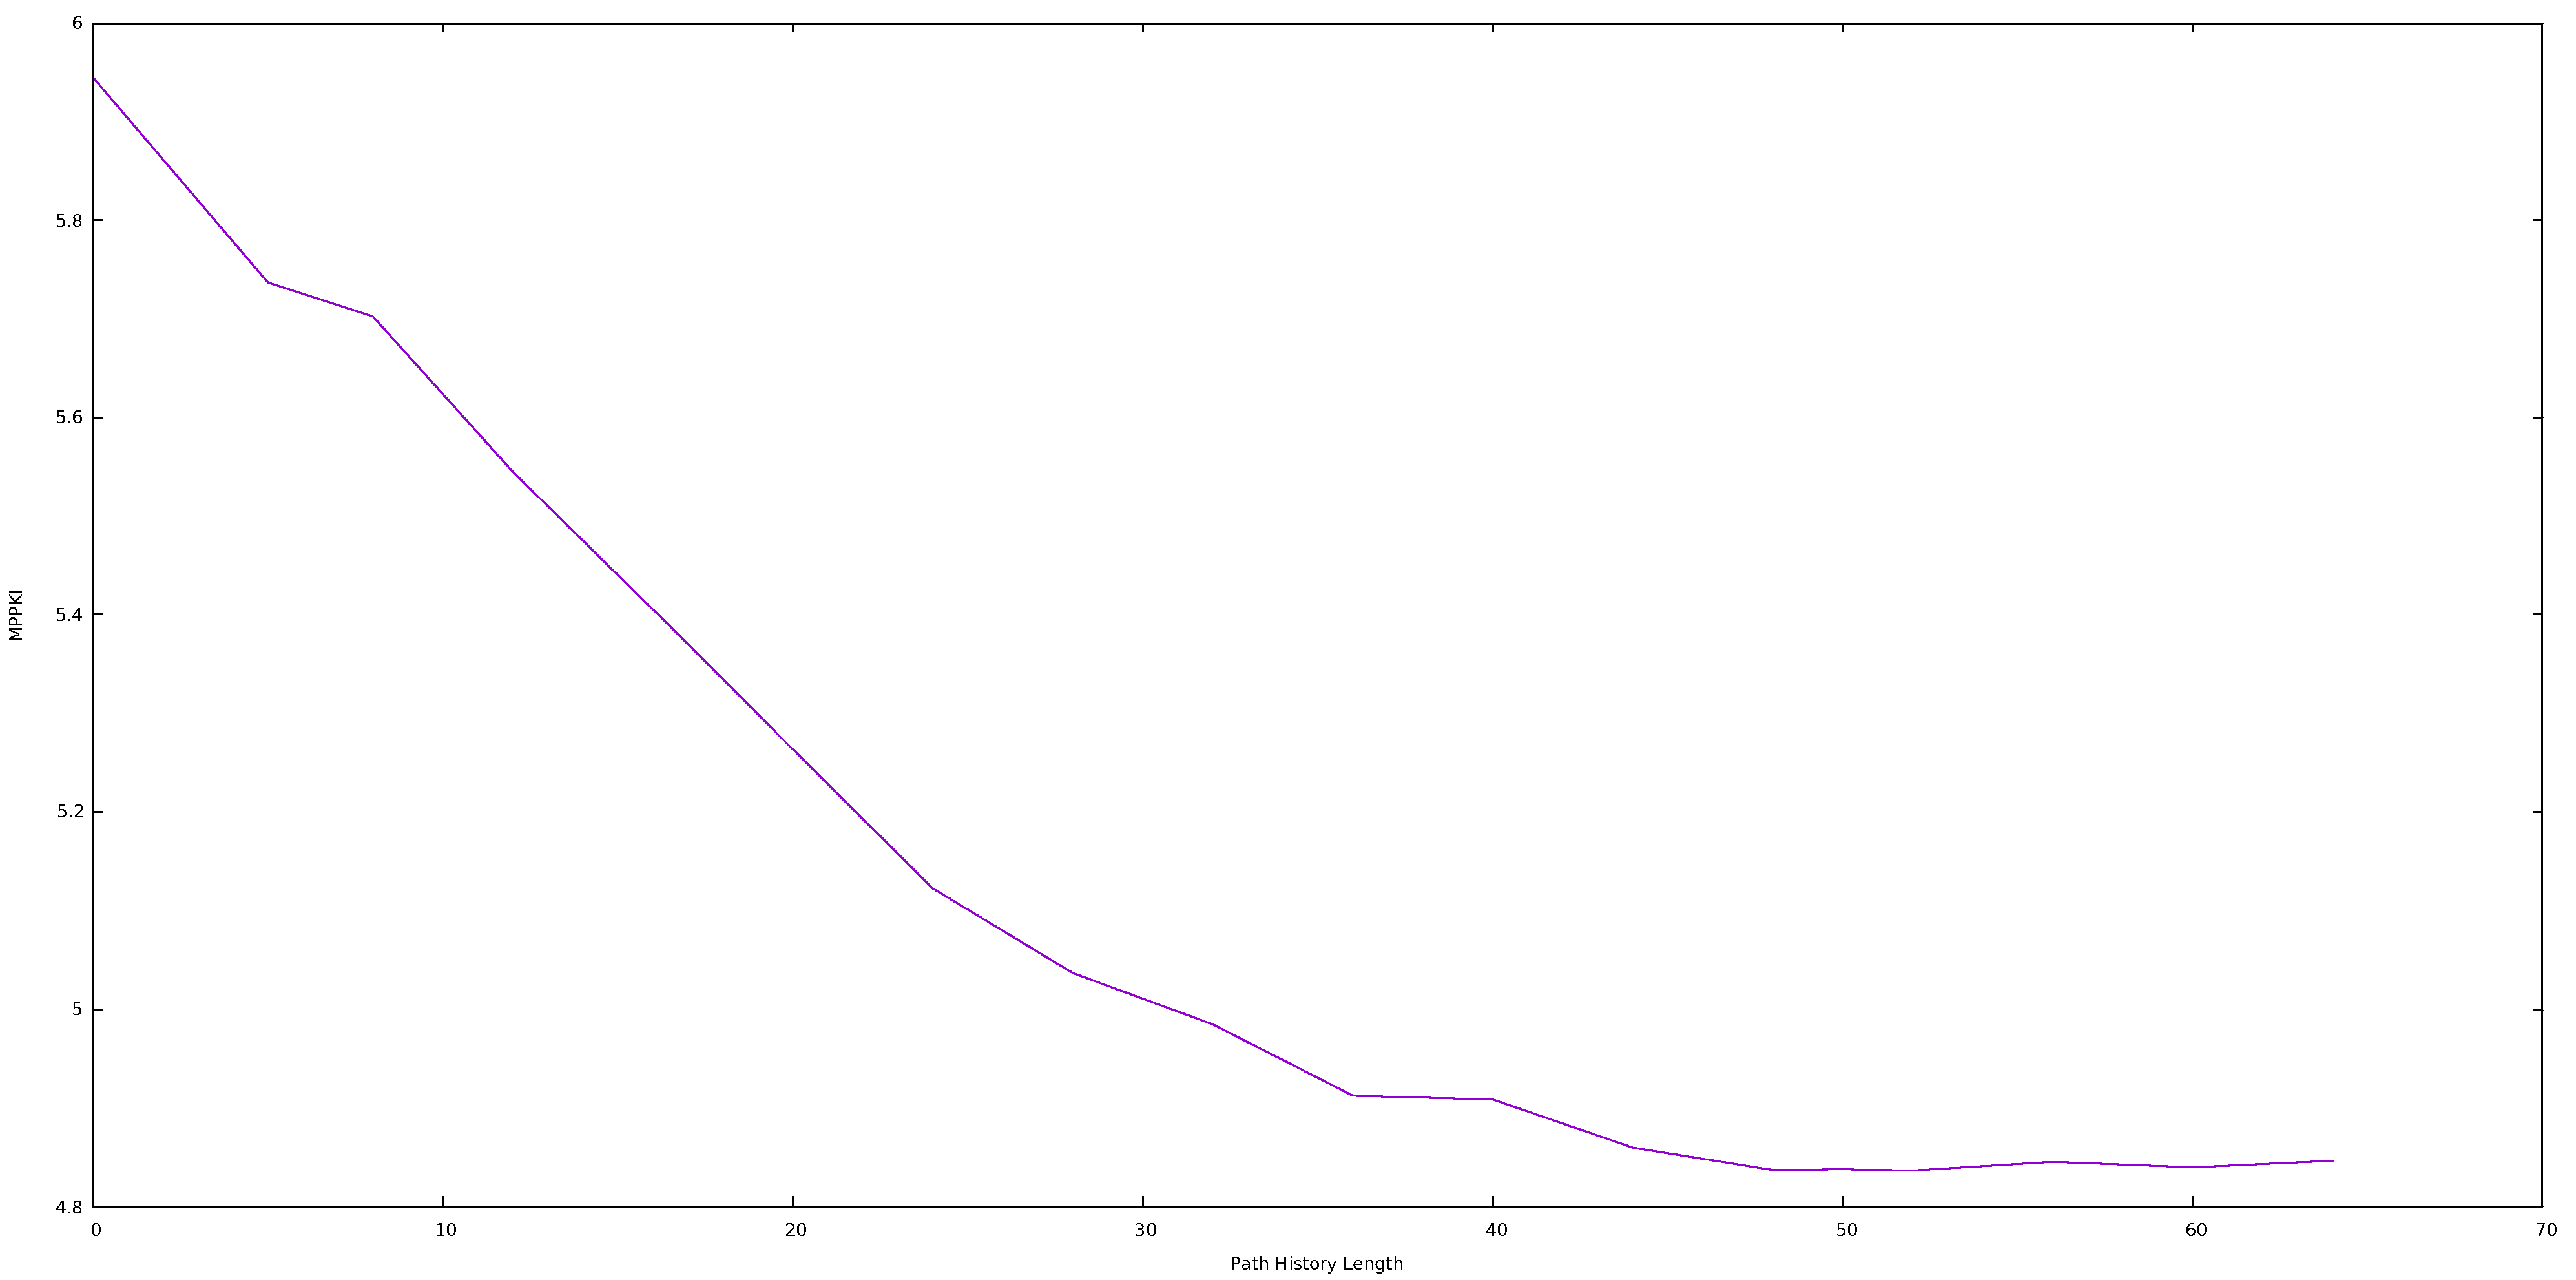
\includegraphics[width=0.45\textwidth]{path-hist}
  \caption{MPPKI vs. Path History Length}
  \label{fig-path-hist}
\end{figure}

We tried various different values for the path history length and arrived at a
value of 48 bits. The results for the different values against the average MPPKI
for the traces can be seen in Figure \ref{fig-path-hist}.

We didn't consider history lengths greater than 64 as path history only effects
short path histories and hence there was no point in trying for greater than 64 bits.

\subsection{Loop Predictor}

The loop predictor provides the global prediction when the loop has successively
been executed 7 times with the same number of iterations. The loop predictor
used in the submission features 32 entries and is 4-way associative. Each entry
consists of a past iteration count on 10 bits, a current iteration count on 10
bits, a partial tag on 12 bits, a confidence counter on 2 bits, a direction bit
and an age counter on 4 bits, i.e. 39 bits per entry. The loop predictor storage
is therefore 1248 bits.

We tried different tag lengths with other parameters remaining the same and a
tag length of 12 gave an optimal value.

Similar, experiments were performed on the confidence counter width and a value
of 2 bits was chosen.

Similar, experiments were performed on the age counter width and a value
of 4 bits was chosen.

The random seed used was adapted from the implementation of randomness in
\cite{ltage}.

\subsection{Threshold}

\begin{figure}[h]
  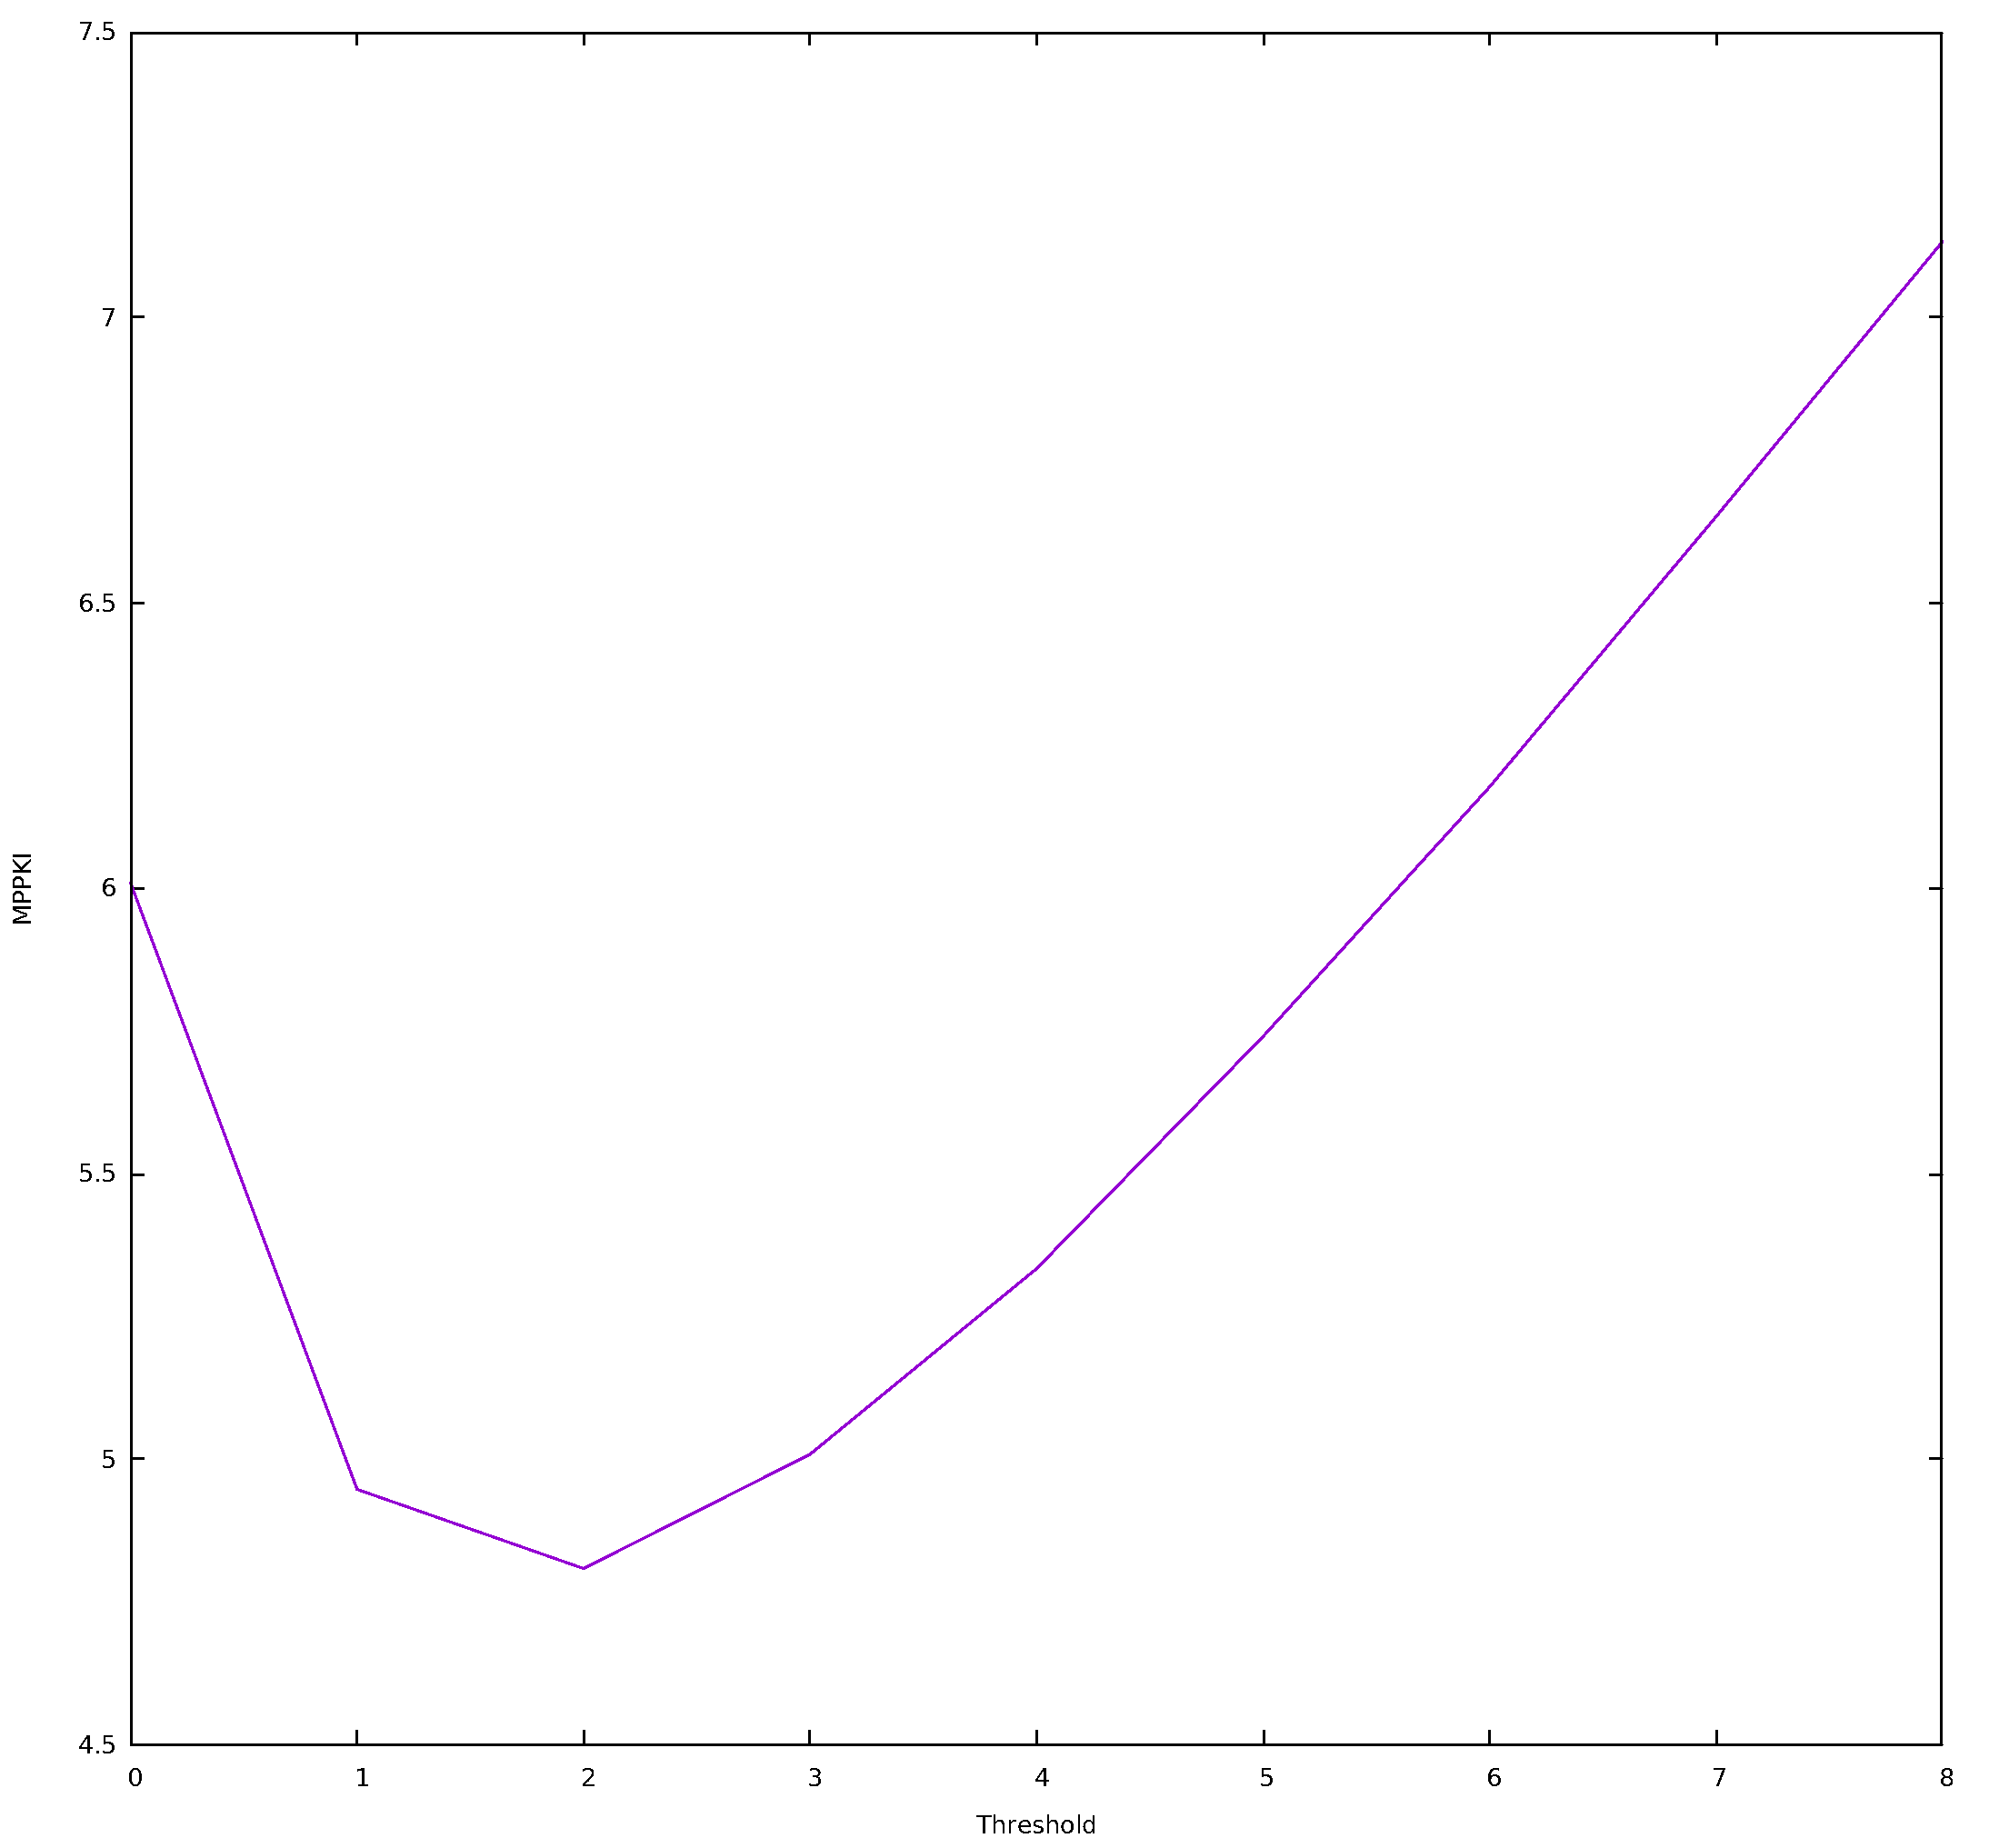
\includegraphics[width=0.35\textwidth]{static-thresh}
  \caption{MPPKI vs. Static Threshold}
  \label{fig-static-thresh}
\end{figure}

\begin{figure}[h]
  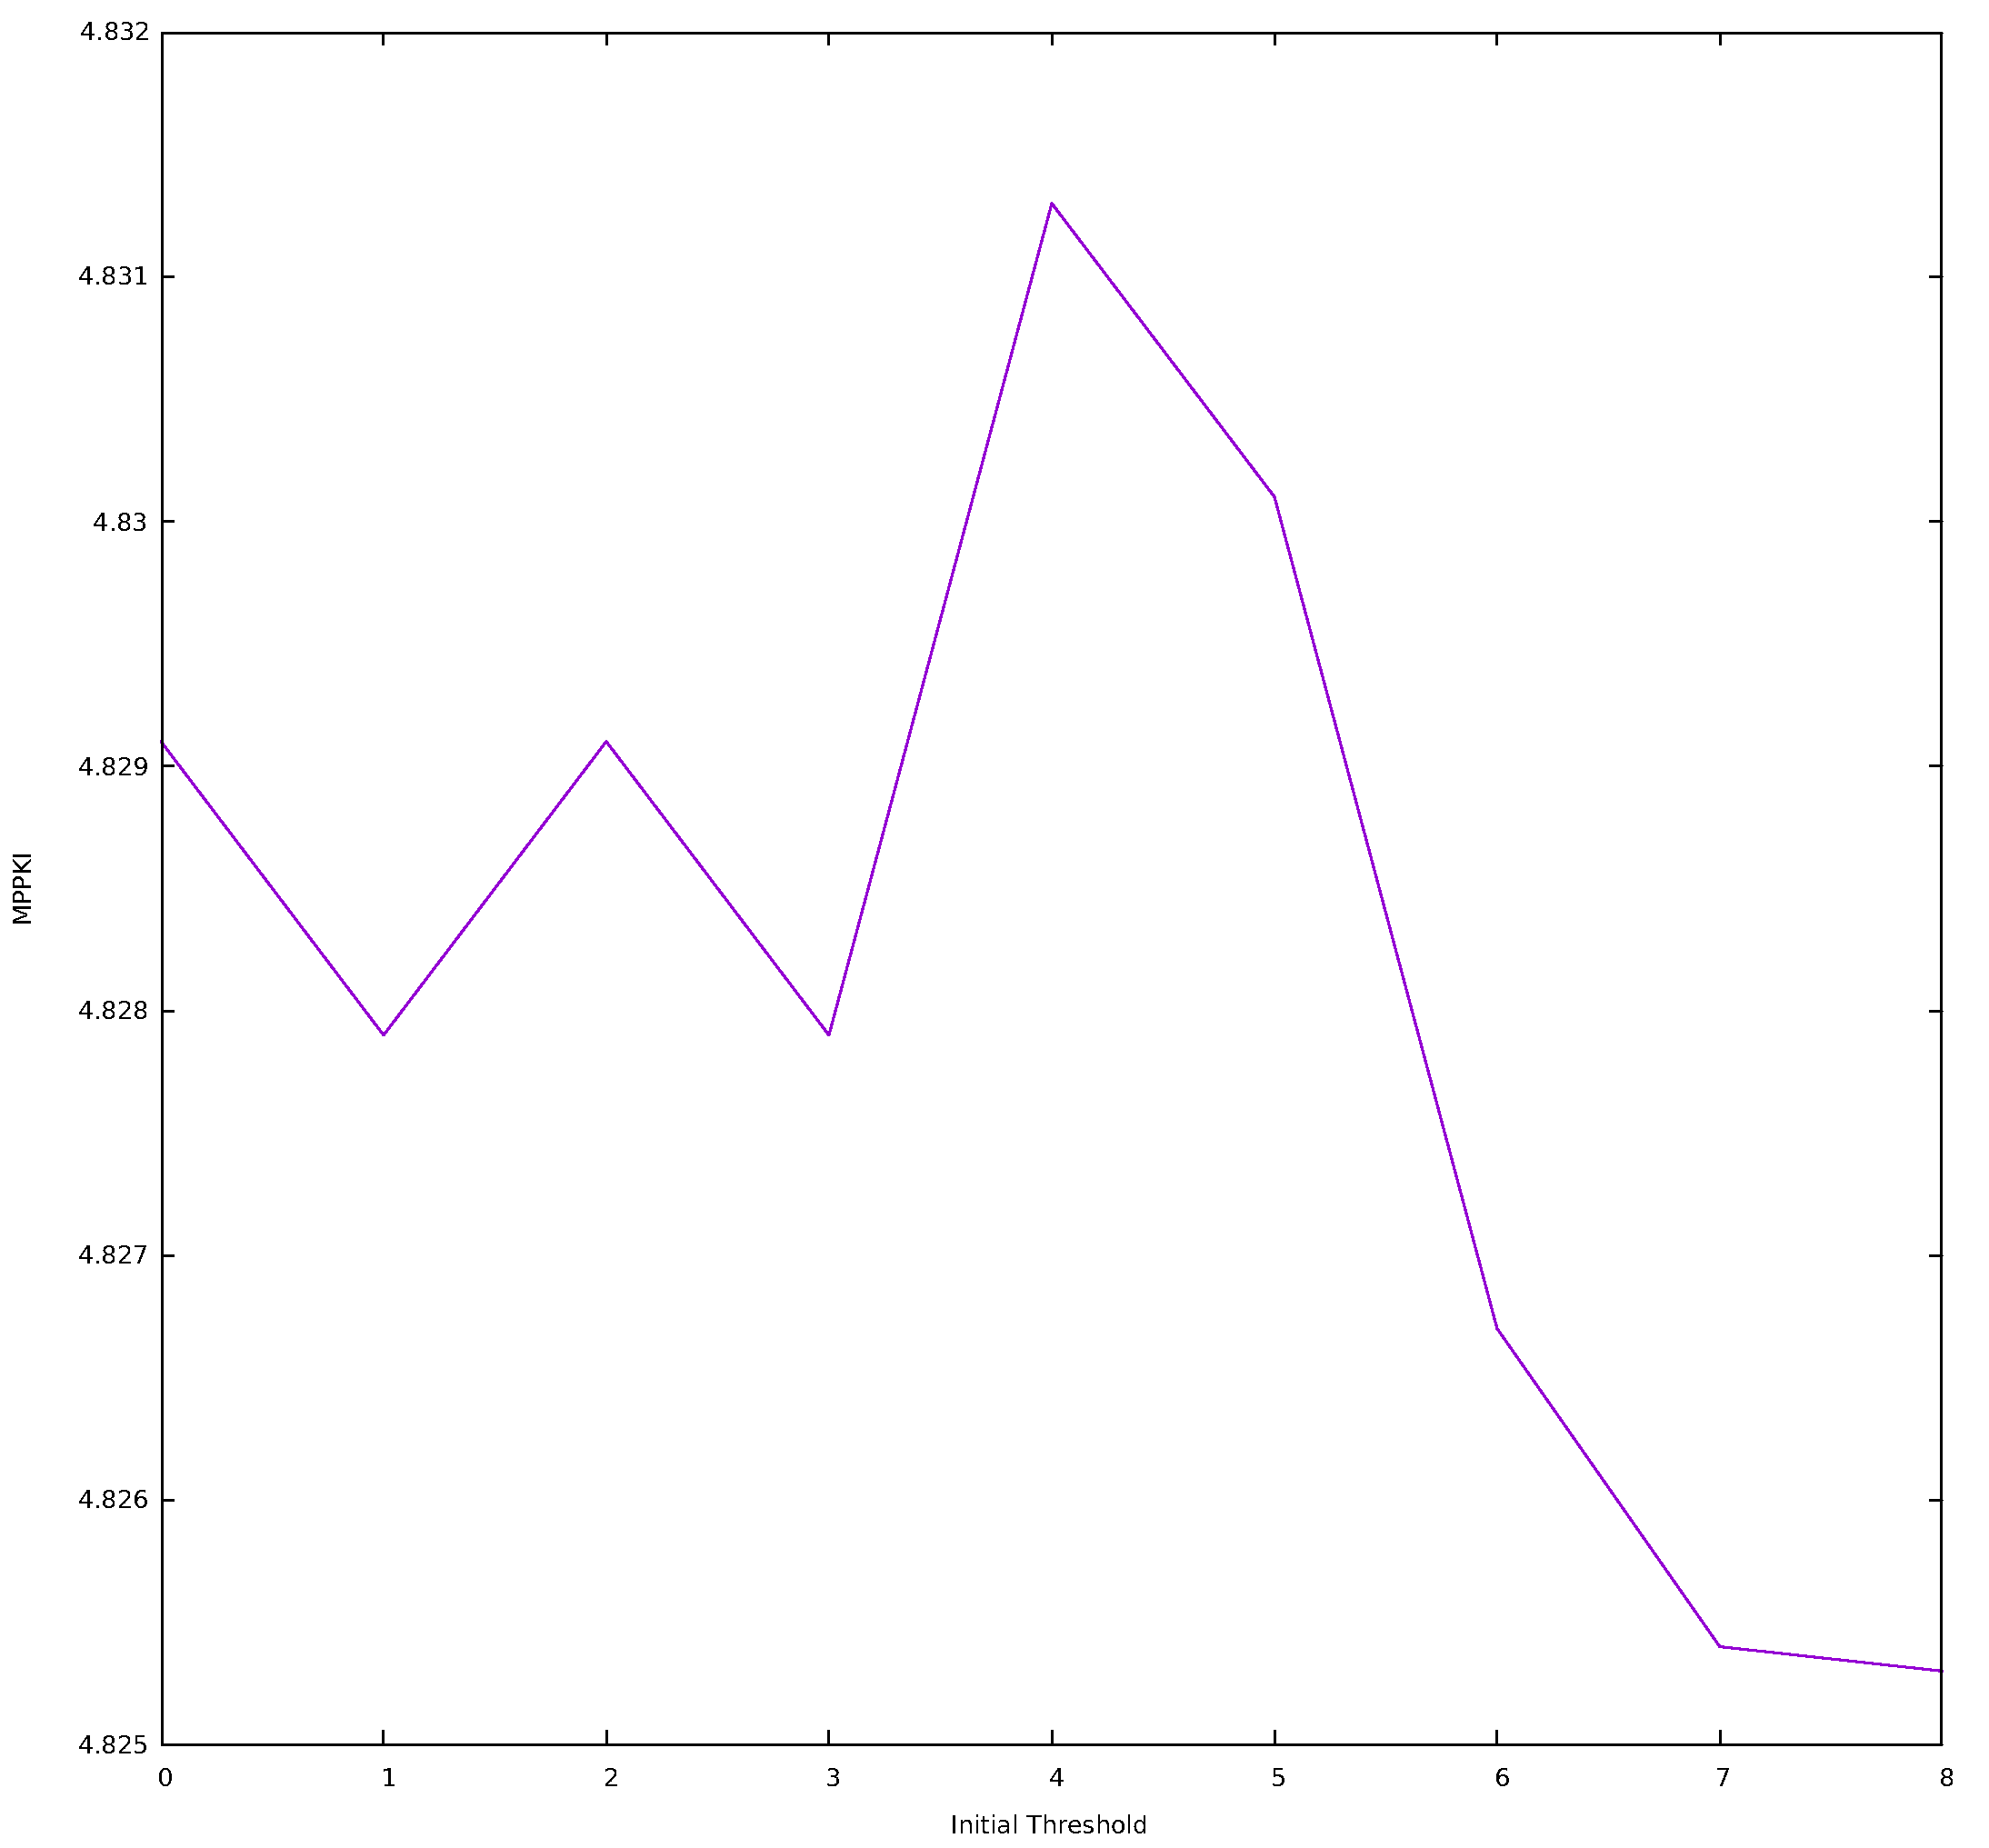
\includegraphics[width=0.35\textwidth]{dyn-thresh}
  \caption{MPPKI vs. Initial Threshold}
  \label{fig-dyn-thresh}
\end{figure}
The results of various static threshold values vs average mppki is in Figure
\ref{fig-static-thresh}.

The results of various initial threshold values in dynamic thresholding vs
average mppki is in Figure \ref{fig-dyn-thresh}.

As can be seen dynamic thresholding easily outperforms static thresholding and
the initial threshold value doesn't affect the results very much in case of
dynamic thresholding.

From the graph, the value for dynamic threshold was chosen to be 8, i.e.,
NUM\_TABLES.

\subsection{Total Hardware Cost}

\begin{center}
  \begin{tabular}{ | c | c | }
    \hline
    Component & Cost \\
    \hline
    Tables & 63K \\ 
    Loop Predictor & 1248 \\  
    Global History & 128 \\
    Pattern History & 48 \\
    WITHLOOP Counter & 7 \\
    THRESH & 3 \\
    TC Counter & 7 \\
    Random Seed & 32 \\
    \hline
    Total & 65985 \\
    \hline
  \end{tabular}
\end{center}

The above value is lesser than the total budget of 64K + 512 bits = 66048
\section{Summary}
\label{sec-summary}

The average MPPKI for the given gshare implementation \cite{combine-bp} is 8.2544

The average MPPKI for our predictor is 4.8253

The average MPPKI of the winner of the first cbp \cite{cbp1.1} on our traces is 5.0266

So our predictor outperforms the winner of the 1st cbp on the given traces on
which we evaluated it.

The work distribution is given in Table \ref{table-work-dist}.

We used \cite{Tange2011a} for generating outputs in parallel and gnuplot for
plotting the results.

\begin{table}[h!]
  \centering
  \begin{tabular}{| c | c |} 
    \hline
    Author & Percentage \\ [0.5ex] 
    \hline
    Subhdeep & 40 \\ 
    Yash & 60 \\ 
    \hline
  \end{tabular}
  \caption{Work Distribution}
  \label{table-work-dist}
\end{table}

%%%%%%% -- PAPER CONTENT ENDS -- %%%%%%%%

%%%%%%%%% -- BIB STYLE AND FILE -- %%%%%%%%
\bibliographystyle{ieeetr}
\bibliography{ref}
%%%%%%%%%%%%%%%%%%%%%%%%%%%%%%%%%%%% 

\end{document}
